\documentclass[10pt,a4paper]{article}

\usepackage[utf8]{inputenc}		% Configuro la codificación
\input{.command.tex}
% En el siguiente archivo se configuran las variables del trabajo práctico
%% \providecommand es similar a \newcommnad, salvo que el primero ante un
%% conflicto en la compilación, es ignorado.
% Al comienzo de un TP se debe modificar los argumentos de los comandos

\providecommand{\myTitle}{TRABAJO FINAL}
\providecommand{\mySubtitle}{Comparación entre HE y ACE}

\providecommand{\mySubject}{Procesamiento de imágenes (86.56)}
\providecommand{\myKeywords}{UBA, Ingeniería, ace, he, histogram, image}

\providecommand{\myAuthorSurname}{Manso}
\providecommand{\myTimePeriod}{Año 2019 - 2\textsuperscript{ndo} Cuatrimestre}

% No es necesario modificar este %%%%%%%%%%%%%%
\providecommand{\myHeaderLogo}{header_fiuba}
%%%%%%%%%%%%%%%%%%%%%%%%%%%%%%%%%%%%%%%%%%%%%%%%

% Si se utilizan listings, definir el lenguaje aquí
\providecommand{\myLanguage}{matlab}
% Crear los integrantes del TP con el comando \PutMember donde
%%		1) Apellido, Nombre
%%		2) Número de Padrón
%%		3) E-Mail
\providecommand{\MembersOnCover}[0]
{
		\PutMember{Manso, Juan} {96133} {juanmanso@gmail.com}
}

\providecommand{\myGroupNumber}{02}


\Pagebreakfalse		% Setea si hay un salto de página en la carátula
\Indexfalse
\Siunitxtrue			% Si quiero utilizar el paquete, \siunixtrue. Si no \siunixfalse
\Todonotesfalse		% Habilita/Deshabilita las To-Do Notes y las funciones \unsure, \change, \info, \improvement y \thiswillnotshow.
\Listingstrue
\Keywordsfalse
\Putgroupfalse		% Habilita/Deshabilita el \myGroup en los headers
\Videofalse
				% Archivo con los comandos globales como Título y autores
%Preambulo para articulo científico de LaTeX

\usepackage[a4paper,left=3cm,right=3cm,bottom=2.5cm,top=3.5cm]{geometry} 	% Configuro la geometría del papel
%\usepackage{microtype}								% Mejora el "spacing" de las palabras
\usepackage[spanish]{babel} 							% Compatibilizo los signos del español
	\addto\captionsspanish{\renewcommand{\tablename}{Tabla}}		%% Redefino nombres preestablecidos por Babel
	\addto\captionsspanish{\renewcommand{\listtablename}{Índice de tablas}}	%% y así en vez de Cuadro dirá Tabla.
	\addto\captionsspanish{\renewcommand{\figurename}{\texttt{Figura}}}
\usepackage{amsmath, amsfonts, amssymb}						% Entornos matemáticos, fuentes y símbolos
\usepackage{graphicx}								% Necesario para insertar figuras
\usepackage{fancyhdr}								% Para manipular headers y footers
\usepackage[usenames,dvipsnames]{color}						% \color{color deseado} {lo que querés que tenga color}
\usepackage{subcaption}								% Permite captions del tipo 1a, 1b
\usepackage{multirow}								% Para tablas
\usepackage{multicol}
\usepackage{float}
\usepackage{mathtools}
\usepackage{dsfont}									% For \mathds{1} to do the mathbb to numbers

% Para video
\ifVideo
	\usepackage{media9}
	\addmediapath{./../reportes/}
\fi

%\usepackage{times}
%\usepackage{mathtools}
%\usepackage{upgreek} % letras griegas sin cursiva
%\usepackage{cancel}
%\usepackage{rotating}
%\usepackage{tikz}
%\usepackage{pgfplots}
%	\pgfplotsset{compat=1.12}
%	\usetikzlibrary{plotmarks}% matlab2tikz
%\usepackage{grffile}% matlab2tikz
%	\usetikzlibrary{calc,patterns,decorations.pathmorphing,decorations.markings}

\ifListings
	\usepackage{listings}

	\providecommand{\lstinputpath}[1]{\lstset{inputpath=#1}}

%	\input{.lst_default.tex}
	\input{.lst_matlab.tex}
%	\input{.lst_c.tex}
%	\input{.lst_c++.tex}

%	\input{.lst_pseudocode.tex}


\fi

\ifSiunitx
\usepackage{siunitx}											% Unidades: \SI {cantidad} {\unidad} (necesita texlive-science)
	\sisetup{load-configurations = abbreviations}							% Habilita poner \cm en vez de \centi\metre
	\sisetup{output-decimal-marker = {,}}									% Cambia los puntos decimales por comas
	\sisetup{per-mode = fraction}											% Pone las unidades como fracción
	\sisetup{quotient-mode = fraction}
\fi


\ifTodonotes
\usepackage{xargs}
\usepackage[colorinlistoftodos,prependcaption,textsize=tiny]{todonotes}
	\newcommandx{\Juan}[2][1=]{\todo[linecolor=blue,backgroundcolor=blue!25,bordercolor=blue,#1]{#2}}
	\newcommandx{\Mati}[2][1=]{\todo[linecolor=green,backgroundcolor=green!25,bordercolor=green,#1]{#2}} % OliveGreen
	\newcommandx{\Emi}[2][1=]{\todo[linecolor=orange,backgroundcolor=orange!25,bordercolor=orange,#1]{#2}}
	\newcommandx{\unsure}[2][1=]{\todo[linecolor=red,backgroundcolor=red!25,bordercolor=red,#1]{#2}}
	\newcommandx{\thiswillnotshow}[2][1=]{\todo[disable,#1]{#2}}
\fi


\usepackage{booktabs}														% Permite hacer tablas sin separadores en el medio
	\usepackage{placeins}
				\let\Oldsection\section												%% Permite que los flotantes (como figuras) no aparescan
			\renewcommand{\section}{\FloatBarrier\Oldsection}						%% antes o después de su sección correspondiente.
				\let\Oldsubsection\subsection
			\renewcommand{\subsection}{\FloatBarrier\Oldsubsection}
				\let\Oldsubsubsection\subsubsection
			\renewcommand{\subsubsection}{\FloatBarrier\Oldsubsubsection}
\usepackage{hyperref}														% Debe ser agregado al final del preambulo

\hypersetup
{			bookmarks=true,         % show bookmarks bar?
			unicode=false,          % non-Latin characters in Acrobat’s bookmarks
			pdftoolbar=true,        % show Acrobat’s toolbar?
			pdfmenubar=true,        % show Acrobat’s menu?
			pdffitwindow=false,     % window fit to page when opened
			pdftitle={\myTitle},    		 % title
			pdfauthor={\myAuthorSurname},   % author
			pdfcreator={\myAuthorSurname},	 % creator = author
			pdfsubject={\mySubject},		 % subject of the document
			pdfkeywords={\myKeywords},
			colorlinks=true,        % false: boxed links; true: colored links
			linkcolor=black,        % color of internal links (change box color with linkbordercolor)
			citecolor=black,        % color of links to bibliography
			filecolor=magenta,      % color of file links
			urlcolor=cyan           % color of external links
}

%Configuro la pagina con los encabezaos y pies de paginas
\pagestyle{fancy}										% Para agregar encabezados y pie de paginas
\lhead{\mySubject}										% Encabezado izquierdo
\rhead{\includegraphics[scale=0.15]{\myHeaderLogo}} 	% Encabezado derecho (logo de la FIUBA)
\ifPutgroup
\chead{\texttt{Grupo Nº\myGroupNumber} }%\\ \textit{\footnotesize{\myTimePeriod}}}
\fi

%% Este archivo contiene las funciones auxiliares para escribir en LaTeX
%% Dichas funciones resuelven la sintaxis de generar figuras, por ejemplo,
%% dejando el código más compacto y facilitando la corrección del mismo.

\newenvironment{MulticolFigure}
	{\par\medskip\noindent\minipage{\linewidth}}
	{\endminipage\par\medskip}

\providecommand{\graficarMulticolPNG}[3]{
			\begin{MulticolFigure}
				\centering
				\includegraphics[width=1.0\textwidth,keepaspectratio]{#1}
					\captionof{figure}{\emph{#2}}
					\label{#3}
			\end{MulticolFigure}

}


% Not working as a command, but yes as a snippet
\providecommand{\graficarMulticolSubfigurePNG}[7]{
	\noindent
	\begin{minipage}{\columnwidth}
		\makeatletter
		\newcommand{\@captype}{figure}
		\centering
			\subfloat[\emph{#2}]{%
				\includegraphics[width=1.0\textwidth]{#1}%
				\label{#3}%
			}\qquad%
			\subfloat[\emph{#5}]{%
				\includegraphics[width=1.0\textwidth]{#4}%
				\label{#6}%
			}
		\caption{\emph{#7}}
	\end{minipage}
}

% Comando para graficar eps. 1er arg, escala. 2do, ruta. 3ro, caption. 4to, label.
\providecommand{\HgraficarEPS}[4]{
			\begin{figure}[h!]
				\centering
					\scalebox{#1}{\input{#2}}
					\caption{#3}
					\label{#4}
			\end{figure}

}

\providecommand{\HgraficarPNG}[4]{
			\begin{figure}[h!]
				\centering
					\includegraphics[scale=#1]{#2}
					\caption{#3}
					\label{#4}
			\end{figure}

}


% Comando para graficar eps en el lugar previsto.
\providecommand{\graficarEPS}[4]{
			\begin{figure}[h]
				\centering
					\scalebox{#1}{\input{#2}}
					\caption{#3}
					\label{#4}
			\end{figure}

}

\providecommand{\graficarPNG}[3]{
			\begin{figure}[h]
				\centering
%					\includegraphics[scale=#1]{#2}
		\includegraphics[width=1.0\textwidth,keepaspectratio]{#1}
					\caption{#2}
					\label{#3}
			\end{figure}

}

\providecommand{\graficarPDF}[3]{
			\begin{figure}[h!]
				\centering
		\includegraphics[width=1.0\textwidth,keepaspectratio]{#1}
					\caption{#2}
					\label{#3}
			\end{figure}

}


\providecommand{\graficarPDFwide}[3]{
			\begin{figure}[h!]
				\centering
		\includegraphics[scale=0.5,trim={6,5cm 0 0 0}]{#1}
					\caption{#2}
					\label{#3}
			\end{figure}

}

\providecommand{\graficarPDFa}[4]{
			\begin{figure}[h!]
				\centering
				\includegraphics[scale=0.5,trim={#1}]{#2}
					\caption{#3}
					\label{#4}
			\end{figure}

}



\providecommand{\underuparrow}[2]{\underset{\underset{#2} \uparrow} #1 }

\providecommand{\cltext}[2]{\color{#1}{\huge{#2}}}

\providecommand{\cstext}[2]{\color{#1}{\large{#2}}}

\providecommand{\vect}[1]{\boldsymbol{#1}}
\providecommand{\dvect}[1]{\dot{\boldsymbol{#1}}}
\providecommand{\dd}{\mathrm{d}}
		% Se proveen un conjunto de funciones extras

% Defino el path de los includegraphics
\graphicspath{{./Figuras/}}		% Directorio que contiene los graficos

% Defino el path para los input de .tex y de .eps
\makeatletter
\def\input@path{{./Figuras/}{./Secciones/}{./Cover_page/}}
\makeatother

% Defino el path del listings
\ifListings
%% Cambiar el nombre de la carpeta si se utilizan Listings
	\lstinputpath{{../code/}}
\fi

\definecolor{myred}{rgb}{0.5,0,0}
\definecolor{mygreen}{rgb}{0,0.5,0}

%\renewcommand{\thesubsection}{\thesection.\alph{subsection}}

\begin{document}
		% Carátula (formal o simple,_formal o _simple respectivamente) con Resumen
		% incluido e Índice (si es necesario configurar en config.tex) del informe
		

% Configuro la carátula


		\title{{\Large{\textbf{\myTitle}}} \\
				\vspace{0.4cm}
				\normalsize\underline{\textbf{\mySubtitle}} \\
		\author{\small{\textsc{\mySubject}}}}
		\date{\small{\myTimePeriod}}
	\maketitle


\ifPutgroup
	\begin{tabbing}
\hspace{6.7cm}\=\+\texttt{Grupo Nº\myGroupNumber}\hspace{5cm}\=
	\end{tabbing}
\fi
	\begin{tabbing}

		\hspace{2cm} \MembersHeader
		
		\newline \vspace{1cm}
		\MembersOnCover

	\end{tabbing}

%	\begin{abstract}
%		
El objetivo del presente trabajo es el estudio del cálculo de coeficientes LPC para el análisis de señales de habla como también para la codificación de las mismas.

%	\end{abstract}	



\ifKeywords
	\begin{center}
		\emph{Palabras Clave: \myKeywords}
	\end{center}
\fi


\noindent\makebox[\linewidth]{\rule{\textwidth}{1pt}} 


\ifPagebreak
	\pagebreak
\fi
	\ifIndex
		\tableofcontents
%		\listoffigures
%		\listoftables
	\fi

\ifPagebreak
	\pagebreak
\fi




	\setcounter{page}{1}

	\renewcommand{\thesection}{\Roman{section}}
	\begin{multicols}{2}

	{\centering\section{Introducción}}
		
En el presente trabajo se analizan dos métodos para la mejora de imágenes
al variar el contraste de las mismas. En clase vimos los métodos de
\emph{streching} y la \emph{ecualización del histograma} o \emph{HE}. El primer
método busca aumentar el rango dinámico del histograma, mientras que el segundo
busca distribuir los valores del histograma (estimación de la función densidad
$f(x)$) de forma tal que la distribución resultante se asemeje a la de una
uniforme. \\

Según el método propuesto por Srinivasan y Balram\footnote{Srinivasan, S
\& Balram, Nikhil. (2006). Adaptive contrast enhancement using local region
stretching.}, la mejora de contraste puede realizarse con ecualizaciones
locales a regiones particulares del histograma ponderadas por una función de
pesos. Esta propuesta (\emph{adaptative contrast enhancement} o \emph{ACE})
muestra ser una mejora a la ecualización del histograma dado que se pueden
obtener resultados que se adapten a la imagen de entrada, resaltando zonas
oscuras o también mejorando el contraste entre objetos.

A continuación se realizará la comparación entre el método \emph{ACE} y el
método \emph{HE}.


	\vspace{0.2cm}
	{\centering\section{Desarrollo}}
		
\subsection{Ecualización de histogramas}

Una variable aleatoria cuya distribución es uniforme tiene la misma probabilidad
de realizarse con un valor, que con cualquier otro. Sin embargo, si se
uniformiza el histograma para que todos los valores de luminancia sean
equiprobables, se perdería la característica de la imagen y el resultado
carecería de sentido en comparación a la original. Es por ello que se
recurre a la linealización de la función de densidad acumulada $F_X(X)$.

De esta manera, al uniformizar la densidad, los picos de luminancia se esparcen
para no quedar concentrados en un rango acotado, aumentando el contraste. \\

Dada una imagen digital de $N$ píxeles con un rango de $M$ valores de luminancia
(típicamente $M=256$) se puede estimar la función densidad de probabilidad de
la luminancia $x$ (\emph{PDF}, \emph{probability density function}) según:

\begin{equation} \label{eq:pdf}
	f(x) = \sum_{i=0}^{M-1} \frac{n_i}{N} \; \mathds{1} \left\{ x = x_i \right\}
\end{equation}

donde $n_i$ corresponde a la cantidad de píxeles cuya luminancia es $x_i$ (que
se limita a $M$ niveles). Éste es el fundamento detrás del uso de histogramas
que representan la \emph{PDF} en un gráfico de barras generado a partir de la
ecuación \eqref{eq:pdf}.

Luego, se obtiene la función de densidad acumulada (\emph{CDF, cumulative
density function}):

\begin{equation} \label{eq:cdf}
	F_X(X) = \sum_{i=0}^{M-1} f(x) \; \mathds{1} \left\{ x \leq x_i \right\}
\end{equation}

Ahora, a partir de la \emph{CDF} calculada en la ecuación \eqref{eq:cdf}, se
realiza el ajuste de la imagen a través de \emph{HE} operando según la siguiente
ecuación para cada píxel ${pix}_i$:

\begin{equation} \label{eq:he_full}
	\textit{HE } ({pix}_i) = \frac{R \; \left[f({pix}_i) - \min\{f(x)\}\right]}{\max\{f(x)\}-\min\{f(x)\}}
\end{equation}

En nuestro caso particular, donde se busca un rango máximo, $R = M - 1 = 255$,
$\max\{f(x)\} = 1$ y $\min\{f(x)\} = 0$. Por lo tanto la ecuación
\eqref{eq:he_full} se puede simplificar:

\begin{equation} \label{eq:he}
	\textit{HE } ({pix}_i) = 255 \cdot f({pix}_i)
\end{equation}

Así, cada valor de luminancia se mapea según su \emph{CDF} a un nuevo valor de
luminancia, manteniendo la posición espacial original.

\graficarMulticolPNG{graph_comp_hist_og_he}{Ejemplo comparativo de histogramas de imágenes con y sin ecualización.}{fig:comp_hist_og_he}

Como se puede ver en la siguiente comparación entre la imagen original y la
ajustada, ésta última realza en exceso el contraste de la imagen generando
efectos indeseados como por ejemplo nubes borrosas de píxeles sobre el personaje
o en los arbustos.

\noindent
\begin{minipage}{\columnwidth}
	\makeatletter
	\newcommand{\@captype}{figure}
	\makeatother
	\centering
		\subfloat[\emph{Original}]{%
			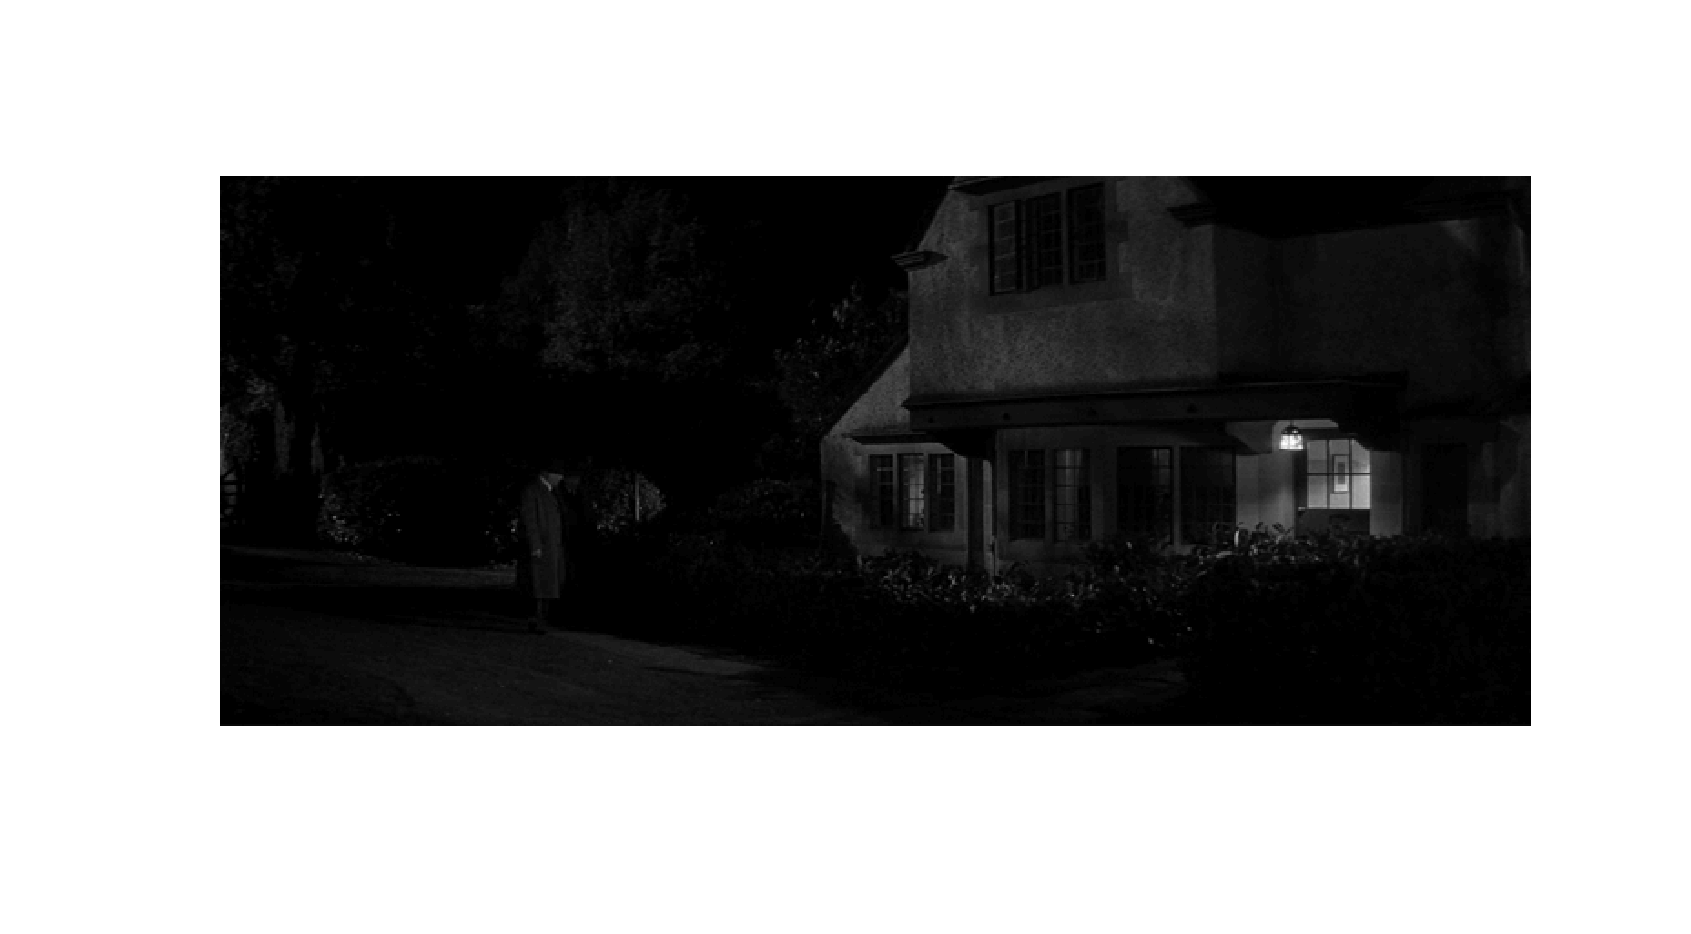
\includegraphics[width=1.0\textwidth]{result_orig_shadowlands}%
			\label{fig:im_orig_he}%
		}\qquad%
		\subfloat[\emph{HE}]{%
			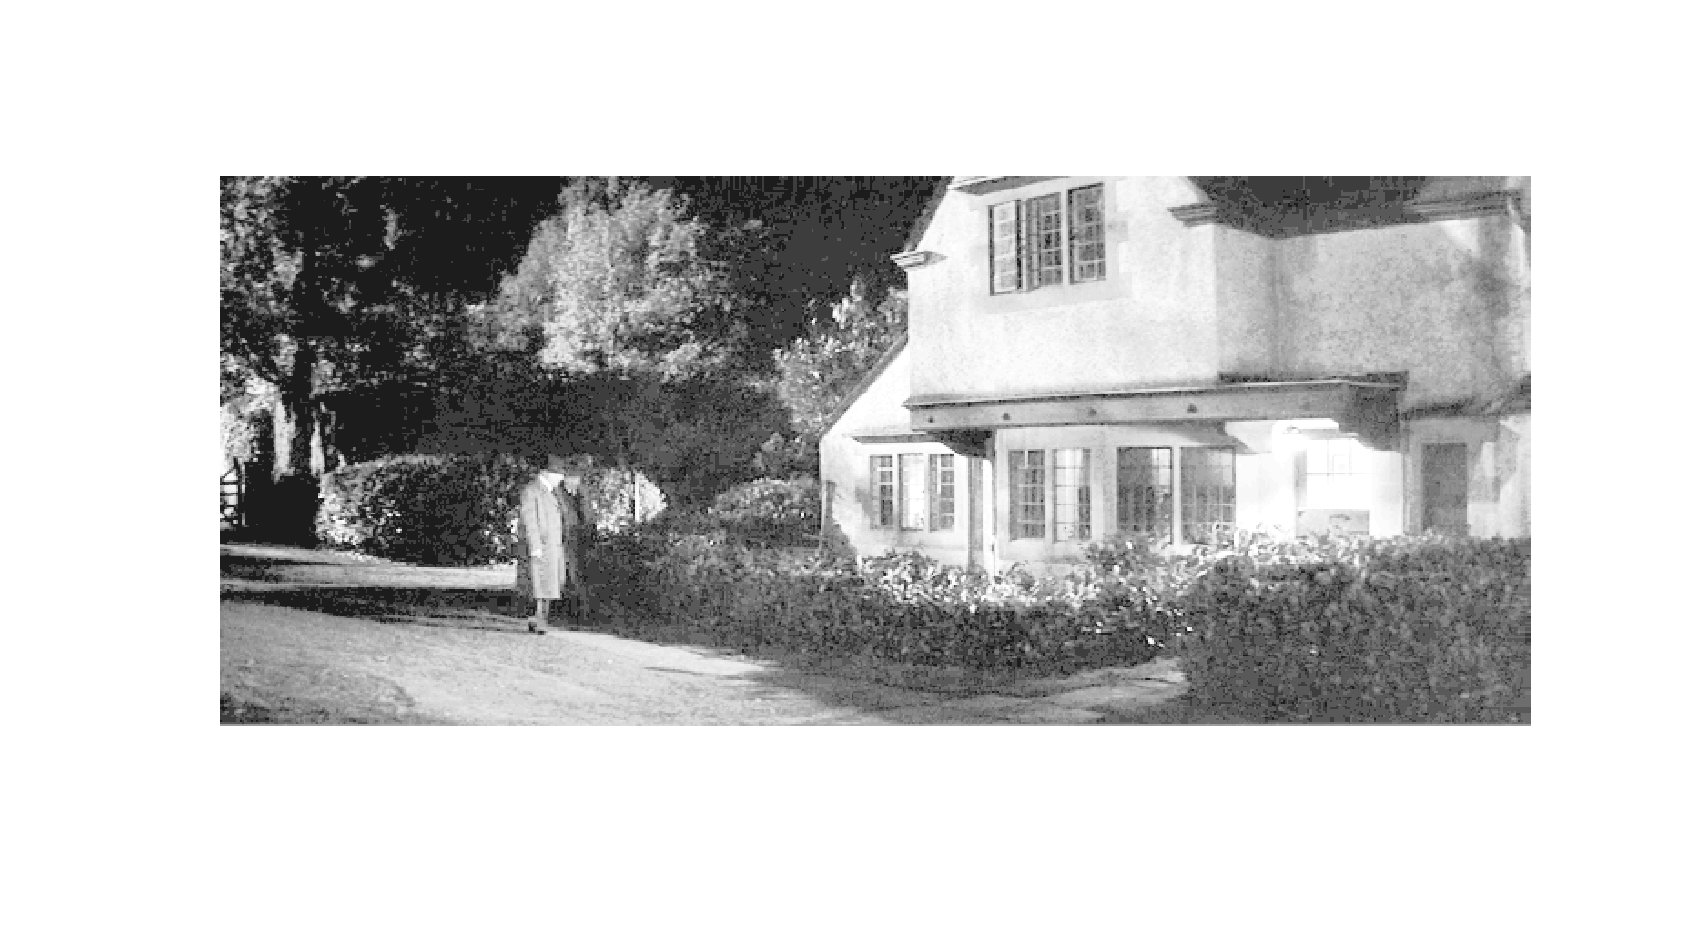
\includegraphics[width=1.0\textwidth]{result_he_shadowlands}%
			\label{fig:im_eq_he}%
		}
	\caption{\emph{Imágenes con y sin HE.}}
\end{minipage}

		\subsection{\emph{Adaptative Contrast Enhancement}}

El método de \emph{Adaptative Contrast Enhancement} toma la técnica de
\emph{HE}, pero la aplica a diferentes regiones del histograma con el objetivo
de disminuir la distorsión generada por el método original. \\

\graficarMulticolPNG{claro_regions}{Diferenciación entre regiones de luminancia
en el histograma de la imagen.}{fig:regiones}

Se definen tres regiones de igual longitud en el histograma basadas en el nivel
de luminancia: oscuro, medio y claro (Figura \ref{fig:regiones}). El método
aplica un \emph{HE} independiente a cada región y luego las une, ponderándolas
según algún criterio a definir.\\

La realización de dicho criterio se encuentra en el factor $w_{i}$ definido para
cada región $i$. El uso de un vector de pesos $W = \begin{bmatrix} w_1 & w_2 & w_3 \end{bmatrix}$
trae dos ventajas fundamentales: mejoras personalizadas para cada caso
particular de imagen y la alternativa de modos de operación. Un caso de uso de los modos
de operación son los filtros provistos por las aplicaciones móbiles para retocar
imágenes para subirlas a las redes sociales. Las mismas aplicaciones suelen tener además
una opción para refinar la imagen de forma más detallada.\\

En el caso más genérico del método, los pesos son calculados a partir de la
pseudo varianza de cada región dadas las medias de luminancia
correspondientes. La varianza da una noción de la forma del histograma, en
particular denota si los puntos se encuentran concentrados en un rango pequeño
de valores o si están dispersos. Analíticamente obtenemos la pseudo varianza
$\sigma_i$ para cada región $i$ según:

\begin{equation} \label{eq:sigma}
	\sigma_i = \frac{1}{N_i} \sum_{j=0}^{m_i} h_j \cdot \left|y_j - \mu_i\right|
\end{equation}

donde, $N_i$ y $m_i$ son la cantidad de píxeles y la cantidad de niveles de
lumniancia dentro del rango $i$ respectivamente. Los valores $h_j$ corresponden
a la cantidad de píxeles cuyo nivel de luminancia es $y_j$ (equivalente al valor
del histograma para $j$). Por último, $\mu_i$ es la media de valores de
luminancia asociado al rango $i$.\\

Habiendo calculado la pseudo varianza para cada rango, se obtienen los pesos a
partir de la siguiente ecuación:

\begin{align} \label{eq:w}
	w_i &= \eta_i \left(1 - \left|\frac{2 \,\sigma_i}{\sigma_{\max}} -1 \right|\right) & \text{con }{\sigma_{\max} = \frac{\max\limits_{\forall j \in \, I}{y_j}}{2}}
\end{align}

con $\eta_i$ siendo un factor de forma determinado por el usuario para
refinamiento de la imagen. El valor de $\sigma_{\max}$ se halla a partir del
peor caso cuya distribución estaría concentrada sólo en los extremos de forma
equiprobable.\\

La ecuación \eqref{eq:w} nace del análisis de comportamiento esperado de los
pesos en función de la pseudo varianza. Para nuestra aplicación, buscamos
asignarle pesos mayores a aquellas regiones cuya pseudo varianza es moderada
porque esto implica que la ecualización generaría poca distorsión. En los casos
extremos (varianza máxima y mínima), la ecualización produciría grandes o nulos
cambios. Gráficamente, la función para calcular los pesos se encuentra en la
Figura \ref{fig:pesos}.

\graficarMulticolPNG{graph_weight_factor}{Función de pesos $w_i$ para cada valor de varianza.}{fig:pesos}

Una vez calculado el vector de pesos, se procede a realizar la ecualización
para cada región. Para ello, se comienza tomando los valores de la función
de densidad acumulada (\emph{CDF}) correspondientes a la región asociada. Luego,
basádonse en la ecuación \eqref{eq:he_full}, se hace el promedio ponderado entre
la ecualizada y la original para la región $i$-ésima según:

\begin{equation} \label{eq:ace}
	\textit{ACE}_i = \textit{orig}_i - w_i \left(\textit{orig}_i - \textit{eq}_i\right)
\end{equation}

Tras la ecualización y la suma ponderada de las regiones, se unen las regiones
obteniendo la imagen adaptada, como se muestra a continuación:

\noindent
\begin{minipage}{\columnwidth}
	\makeatletter
	\newcommand{\@captype}{figure}
	\makeatother
	\centering
		\subfloat[\emph{Original}]{%
			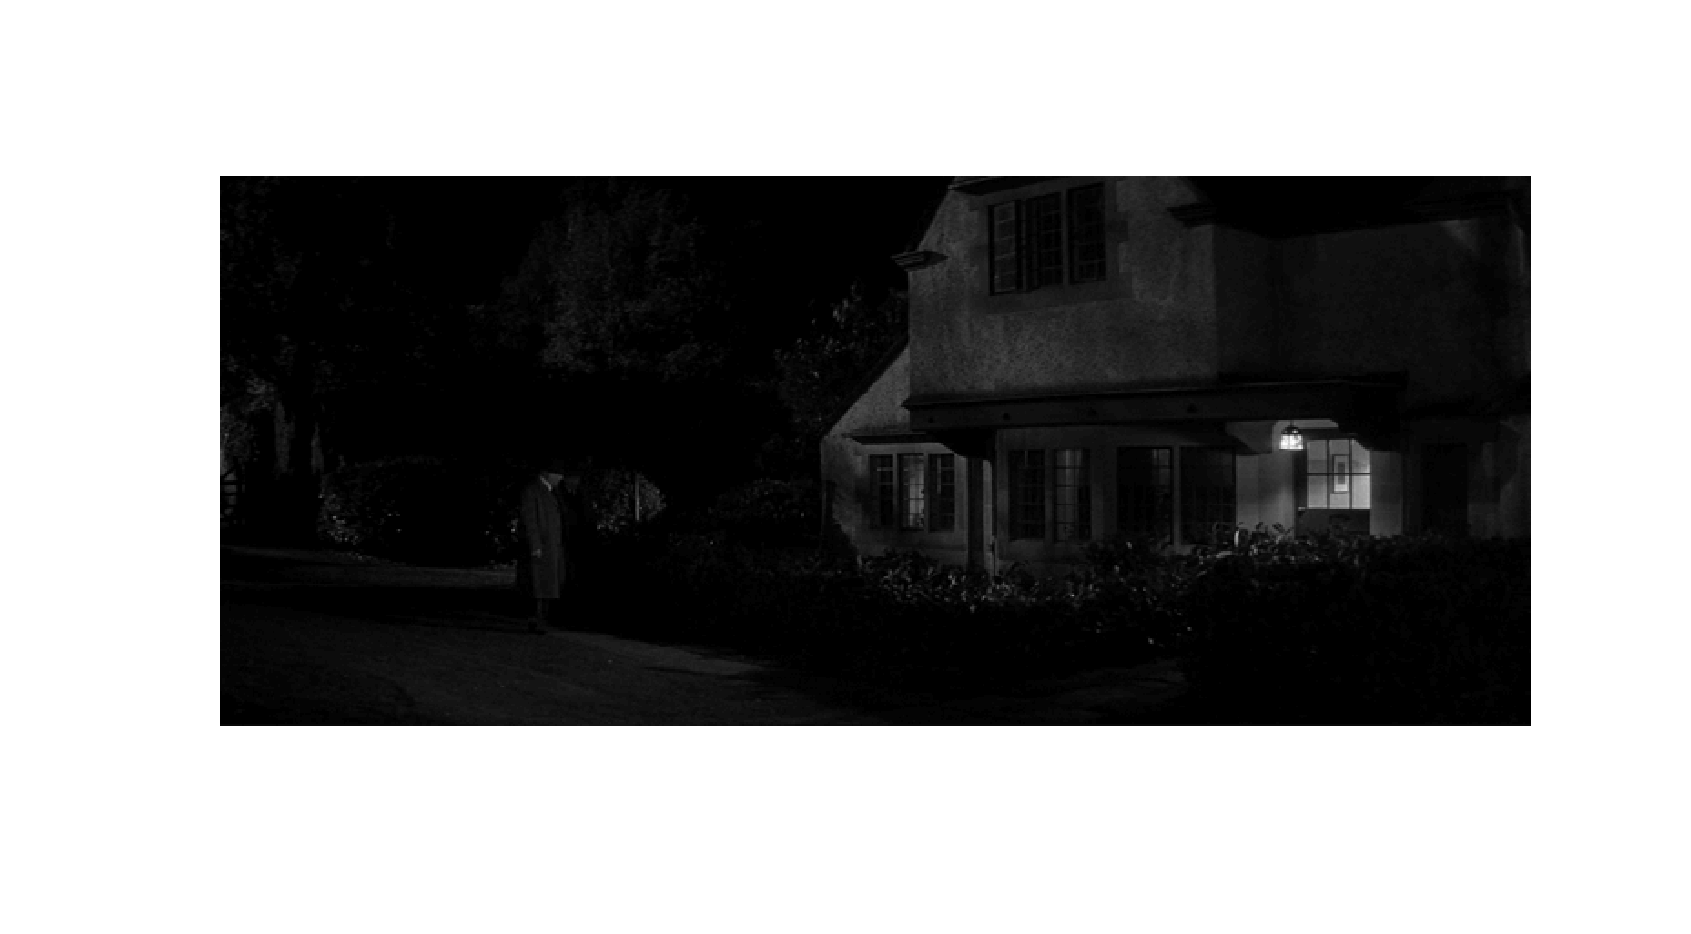
\includegraphics[width=1.0\textwidth]{result_orig_shadowlands}%
			\label{fig:im_orig_ace}%
		}\qquad%
		\subfloat[\emph{ACE}]{%
			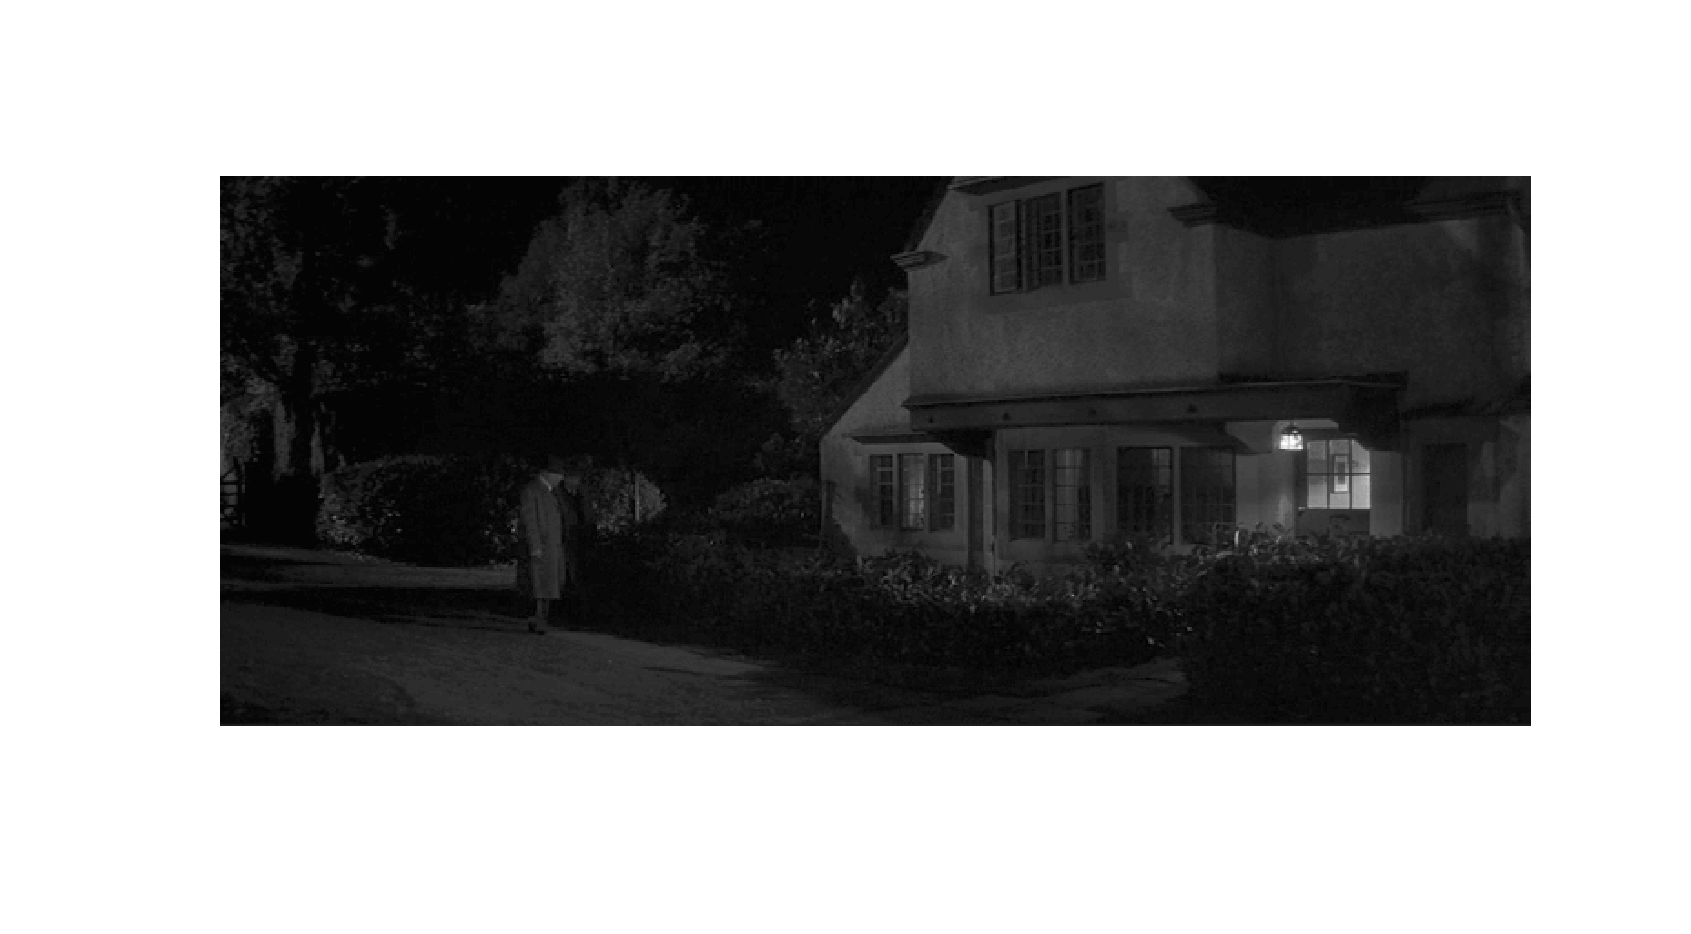
\includegraphics[width=1.0\textwidth]{result_ace_shadowlands}%
			\label{fig:im_ace_ace}%
		}
	\caption{\emph{Comparación entre imágenes con y sin ACE denotando una mejora de contraste entre los objetos.}}
\end{minipage}

		\subsection{\emph{Resultados}}

Para el análisis de la efectividad del método, podemos hacer 3 tipos de
comparaciones:
\begin{enumerate}
	\item Imagen
	\item Histograma
	\item Relación señal-ruido pico ($PSNR$)
\end{enumerate}

\begin{figure*}%
	\centering
		\begin{subfigure}{1.0\columnwidth}
		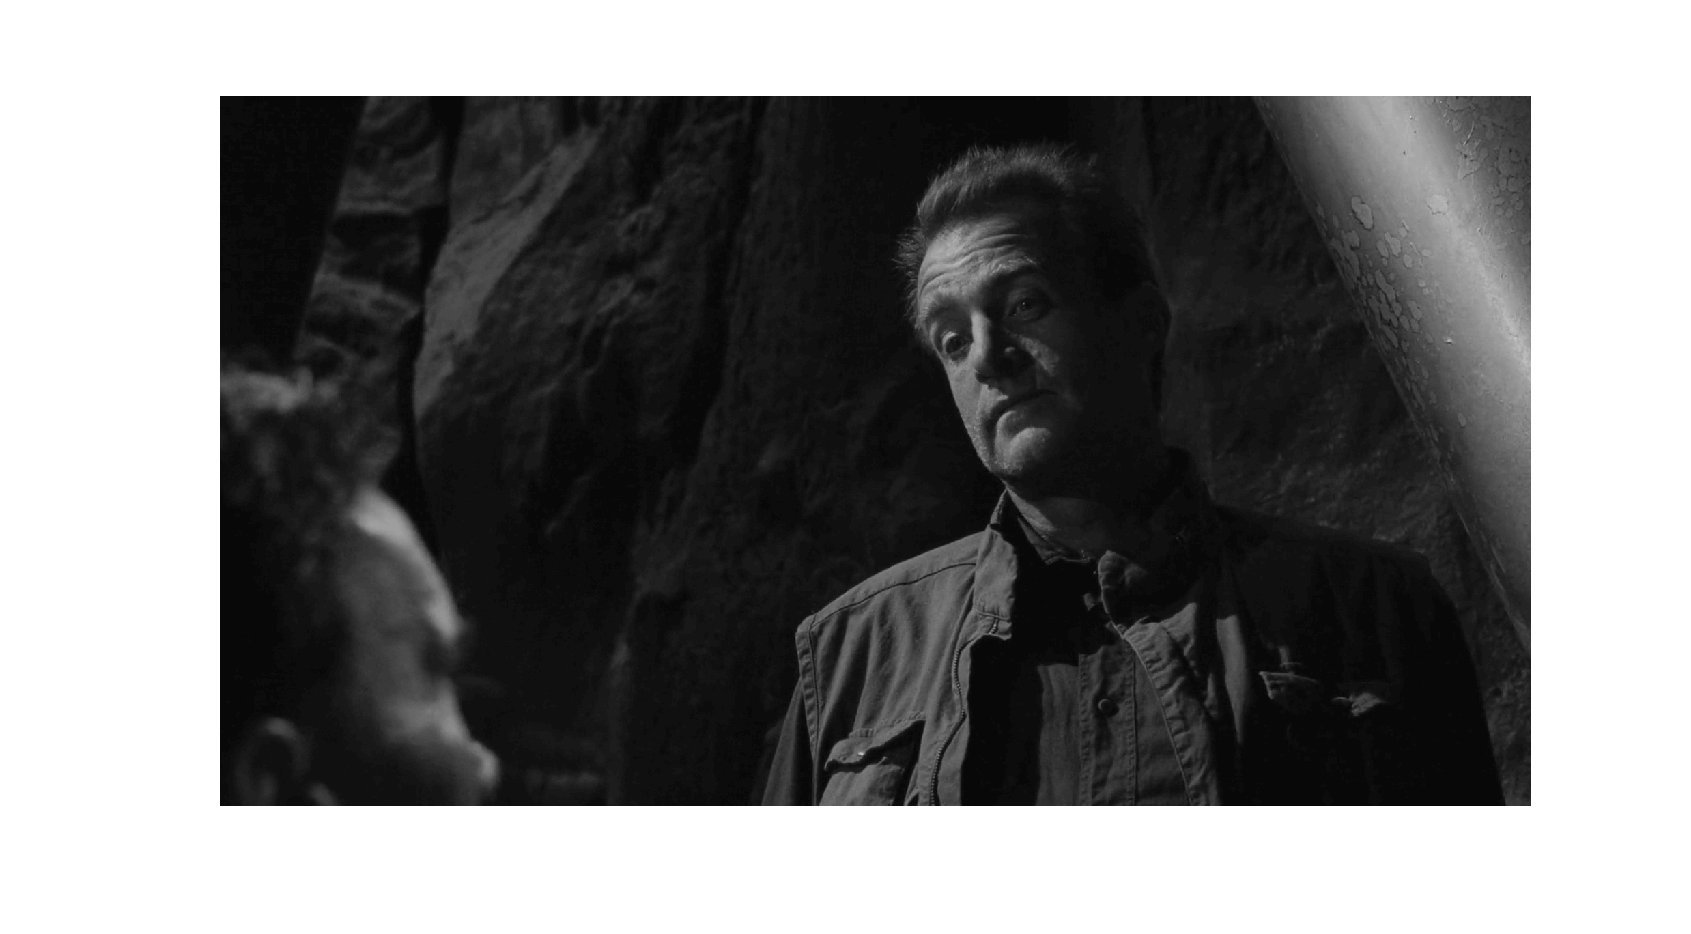
\includegraphics[width=\columnwidth]{result_orig_totalrecall}%
		\caption{Original}%
		\label{subfig:original}%
	\end{subfigure}\hfill%
	\begin{subfigure}{1.0\columnwidth}
		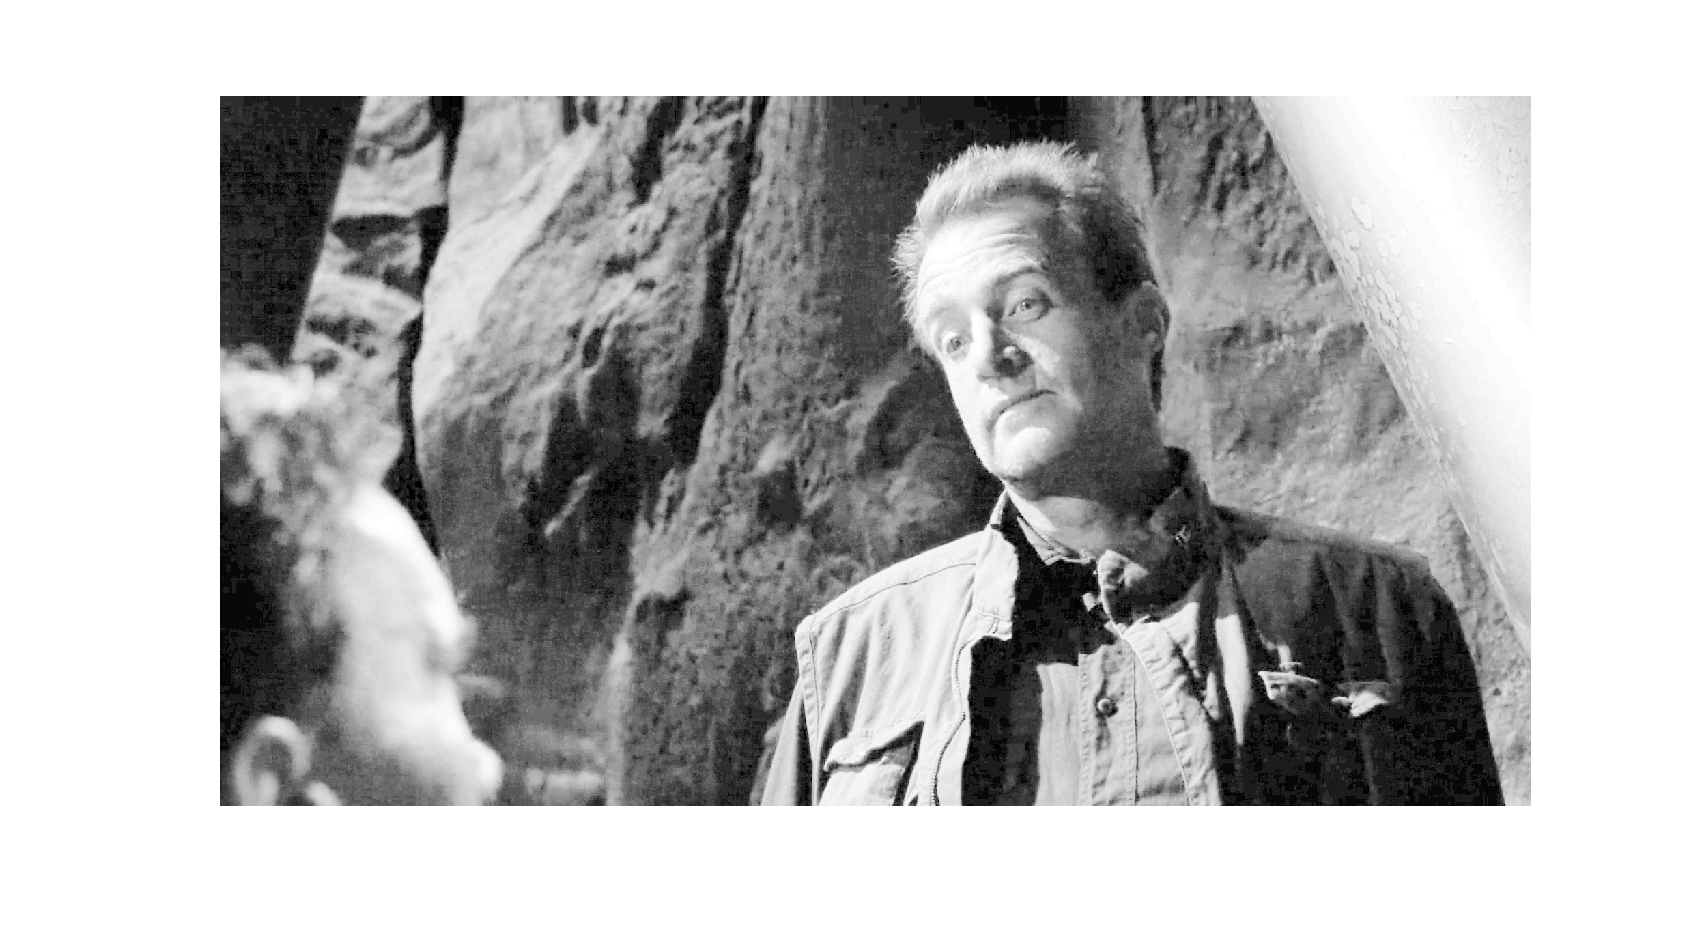
\includegraphics[width=\columnwidth]{result_he_totalrecall}%
		\caption{HE}%
		\label{subfig:he}%
	\end{subfigure}\hfill%
	\begin{subfigure}{1.0\columnwidth}
		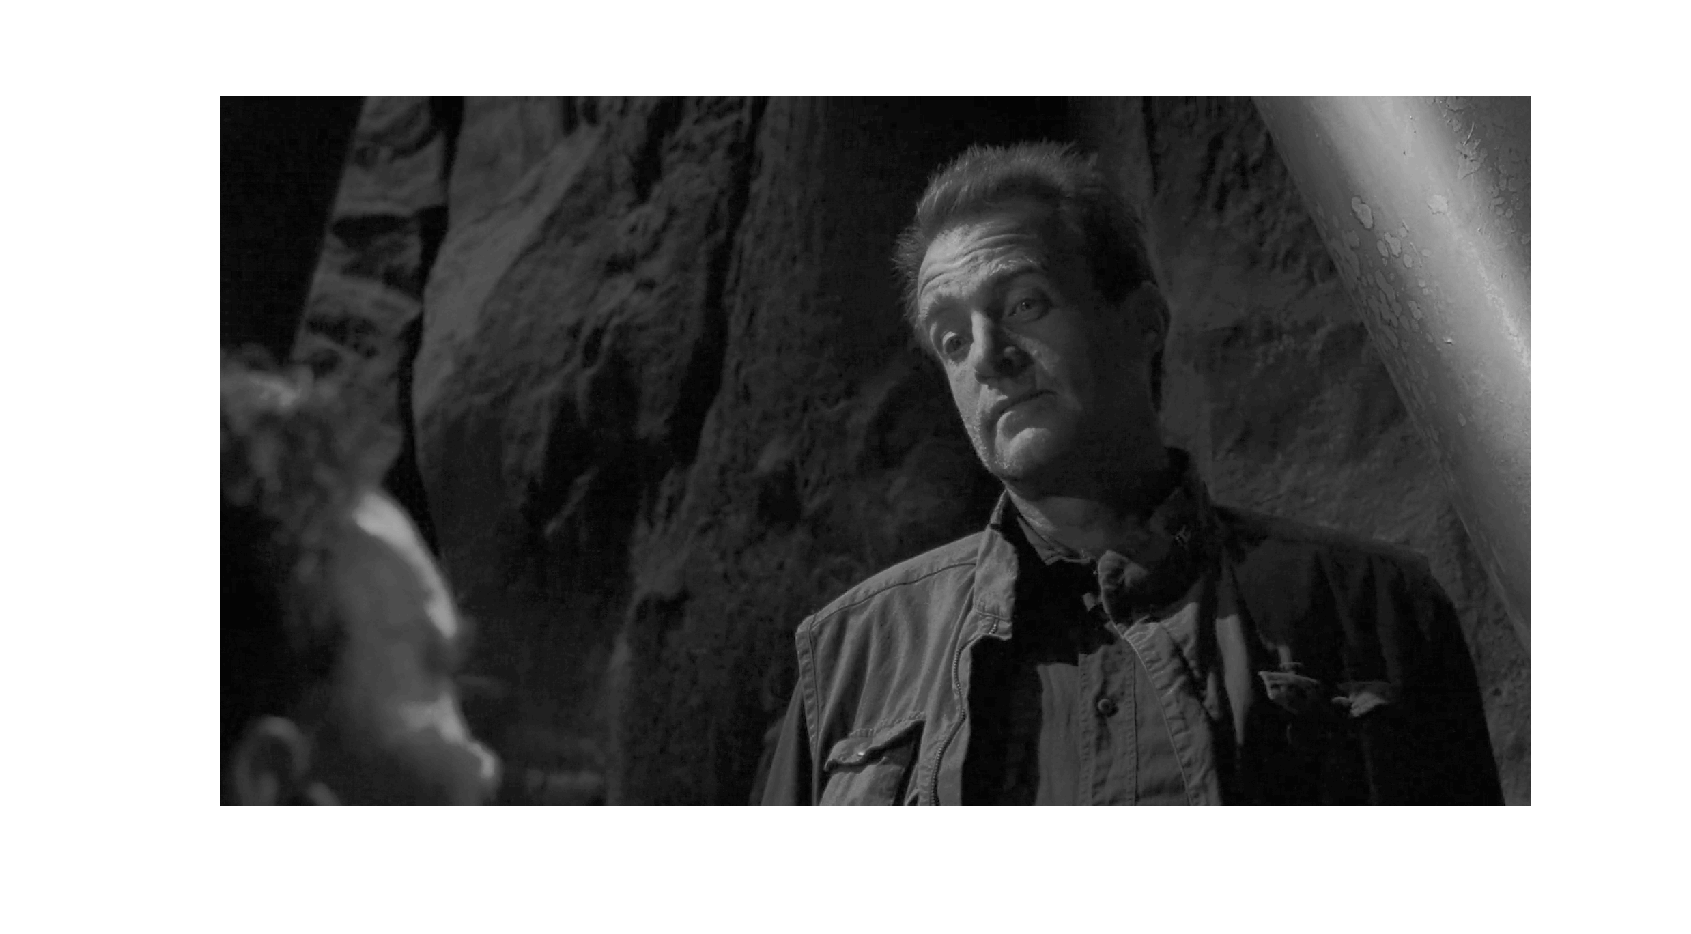
\includegraphics[width=\columnwidth]{result_ace_totalrecall}%
		\caption{ACE}%
		\label{subfig:ace}%
	\end{subfigure}%
	\caption{Comparación de resultados para la imagen de prueba \emph{Total Recall}.}
	\label{fig:comp_imagenes}
\end{figure*}

Como se puede ver en la Figura \ref{fig:comp_imagenes}, la ecualización del
histograma puede generar imágenes saturadas con respecto a las originales
(con Figura \ref{subfig:he} y Figura \ref{subfig:original} respectivamente). En
cambio, al hacer la comparación de la Figura \ref{subfig:original} y la alterada
por $ACE$ (Figura \ref{subfig:ace}), esta última muestra un mejor contraste
visual versus su contraparte de $HE$.\\

Para evaluar la variación del rango dinámico, se hallan los histogramas
correspondientes para cada caso como se puede ver en la Figura
\ref{fig:comp_histo}.

\graficarMulticolPNG{result_comp_hist}{Histograma de las imágenes procesadas por
HE y ACE, en comparación con la original.}{fig:comp_histo}

Como se puede ver en la Figura \ref{fig:comp_histo}, en ambos casos ($HE$ y
$ACE$) el rango dinámico aumenta. Sin embargo, se puede apreciar que el
histograma del $HE$, aunque de  mayor rango, contiene mayor cantidad de
discontinuidades o picos, mientras que el del $ACE$ tiene una envolvente más
suave y concentrada en un rango dado. Esto implica que la imagen modificada por
$HE$ presenta mayores saturaciones, resultando en artefactos indeseados.

Finalmente, en la Tabla \ref{tab:comp_psnr} se hallan los valores de $PSNR$ de
los dos métodos bajo análisis. Queda en evidencia de forma analítica, que
la propuesta de $ACE$ mejora la imagen en mayor medida que el $HE$, al tener un
$PSNR$ mayor en todos los casos. Para la imagen \emph{Shadowlands}, el $MSE$
utilizado para el cálculo de $PSNR$ es tan pequeño que genera un resultado infinito.\\

\noindent
\begin{minipage}{\columnwidth}
	\makeatletter
	\newcommand{\@captype}{table}
	\centering
	\begin{tabular}{@{}ccc@{}}
		\toprule
		Imagen de prueba& ${PSNR}_{he}$ & ${PSNR}_{ace}$ \\
		\midrule
		Total Recall	& $54.524$      & $59.705$       \\
		Shadowlands  	& $\infty$      & $\infty$       \\
		Odín         	& $28.232$      & $32.429$		 \\
		\bottomrule
	\end{tabular}
	\caption{\emph{Peak Signal-to-noise ratio} para las 3 imágenes de prueba}
	\label{tab:comp_psnr}
\end{minipage}



	\vspace{0.2cm}
	{\centering\section{Conclusiones}}
		El método de \emph{Adaptive contrast enhancement} es una buena alternativa al
tradicional método de ecualización del histograma (\emph{HE}) para su aplicación
en video dada su fácil configuración y versatilidad ante imágenes de
variadas características.\\

A pesar de agregar mayor complejidad al método, el mismo provee mejoras
y personalización que justifican su implementación tanto en sistemas
de procesamiento de imágenes como de video.



	\end{multicols}

	\pagebreak
	\appendix
		\section{Imágenes de prueba}
			Para generar las imágenes de prueba con el método ACE, se utilizó un modo de operación uniforme de $\eta^1 = \begin{bmatrix} 0.5 & 0.5 & 0.5\end{bmatrix}$.
			\subsection{Total Recall}
				\HgraficarPNG{0.16}{result_orig_totalrecall}{Imagen Original}{fig:app_og_tr}
				\HgraficarPNG{0.16}{result_he_totalrecall}{Imagen modificada por HE}{fig:app_he_tr}
				\HgraficarPNG{0.16}{result_ace_totalrecall}{Imagen modificada por ACE}{fig:app_ace_tr}
			\subsection{Shadowlands}
				\HgraficarPNG{0.18}{result_orig_shadowlands}{Imagen Original}{fig:app_og_sl}
				\HgraficarPNG{0.18}{result_he_shadowlands}{Imagen modificada por HE}{fig:app_he_sl}
				\HgraficarPNG{0.18}{result_ace_shadowlands}{Imagen modificada por ACE}{fig:app_ace_sl}
			\subsection{Odín}
				\HgraficarPNG{0.18}{result_orig_odin}{Imagen Original}{fig:app_og_od}
				\HgraficarPNG{0.18}{result_he_odin}{Imagen modificada por HE}{fig:app_he_od}
				\HgraficarPNG{0.18}{result_ace_odin}{Imagen modificada por ACE}{fig:app_ace_od}

		\section{Imágenes oscuras con un modo de operación personalizado}
			Si se realizan modificaciones al modo de operación, las imágenes pueden mejorar su contraste considerablemente. En este ejemplo, se utiliza un $\eta^2 = \begin{bmatrix} 0.4 & 0.5 & 0.1\end{bmatrix}$ para concentrar la mejora en las zonas oscuras y medias. El contraste puede disminuir pero también lo hacen los artefactos en la imagen.
			\subsection{Total Recall}
				\HgraficarPNG{0.25}{result_ace_totalrecall}{Imagen modificada por ACE}{fig:app_ace_tr2}
				\HgraficarPNG{0.25}{alt_totalrecall}{Imagen modificada utilizando $\eta^2$}{fig:app_he_alt}
			\subsection{Shadowlands}
				\HgraficarPNG{0.27}{result_ace_shadowlands}{Imagen modificada por ACE}{fig:app_ace_sl2}
				\HgraficarPNG{0.27}{alt_shadowlands}{Imagen modificada utilizando $\eta^2$}{fig:app_he_alt}

		\pagebreak
		\section{Funciones principales}
			\subsection{tpf.m}
				\lstinputlisting[caption = \texttt{tpf.m}]{tpf.m}
			\subsection{ace.m}
				\lstinputlisting[caption = \texttt{ace.m}]{utils/ace.m}
%
		\section{Funciones auxiliares}
			\subsection{cdf.m}
				\lstinputlisting[caption = \texttt{cdf.m}]{utils/cdf.m}
			\subsection{histo.m}
				\lstinputlisting[caption = \texttt{histo.m}]{utils/histo.m}
			\subsection{equalizer.m}
				\lstinputlisting[caption = \texttt{equalizer.m}]{utils/equalizer.m}
			\subsection{weighted\_factor.m}
				\lstinputlisting[caption = \texttt{weighted\_factor.m}]{utils/weighted_factor.m}
			\subsection{psnr.m}
				\lstinputlisting[caption = \texttt{psnr.m}]{utils/psnr.m}
\end{document}
